\documentclass[aspectratio=169]{beamer}

\usepackage{graphicx}
\usepackage{amsmath}
\usepackage{xcolor}
\usepackage{listings}

\setbeamertemplate{navigation symbols}{}

\title{From PCA + Volcano Plots to GO Enrichment}
\subtitle{How we moved from global structure \texorpdfstring{$\rightarrow$}{->} gene-level signals \texorpdfstring{$\rightarrow$}{->} functional summaries}
\author{BIOL550 Mouse RNA-seq}
\date{\today}

\lstset{
  basicstyle=\ttfamily\footnotesize,
  keywordstyle=\color{blue!70!black},
  commentstyle=\color{gray!70!black},
  stringstyle=\color{teal!60!black},
  showstringspaces=false,
  columns=fullflexible,
  frame=single,
  rulecolor=\color{black!20},
}

\begin{document}

\begin{frame}
  \titlepage
\end{frame}

\begin{frame}{PCA first: global structure before gene lists}
\begin{columns}[T,onlytextwidth]
  \column{0.62\textwidth}
  \centering
  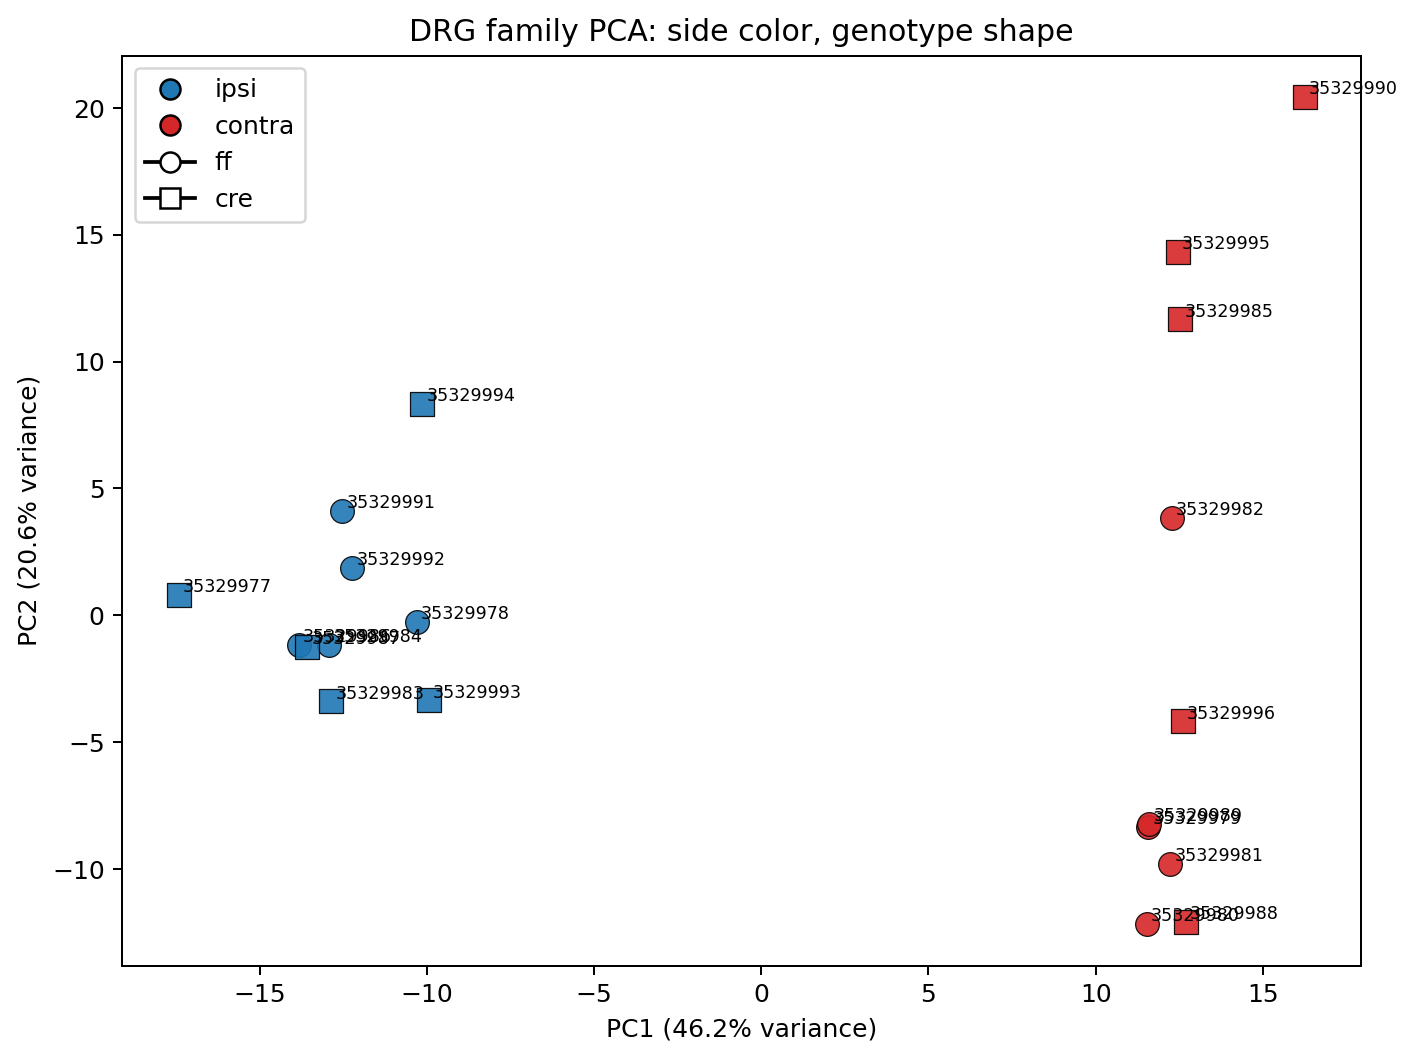
\includegraphics[width=\linewidth]{../data/differential_expression_all20/derived_analysis/family_structure/pca_side_genotype_annotated.png}

  \column{0.38\textwidth}
  \small
  \begin{itemize}
    \item PCA asks: what explains the largest variation in expression across samples?
    \item Use it to sanity-check whether samples separate by biology vs. batch/technical effects.
    \item Then move to gene-level interpretation (volcano / DE tables).
  \end{itemize}
\end{columns}
\end{frame}

\begin{frame}{Too many DE genes: bend-point (elbow) selection}
\begin{columns}[T,onlytextwidth]
  \column{0.70\textwidth}
  \centering
  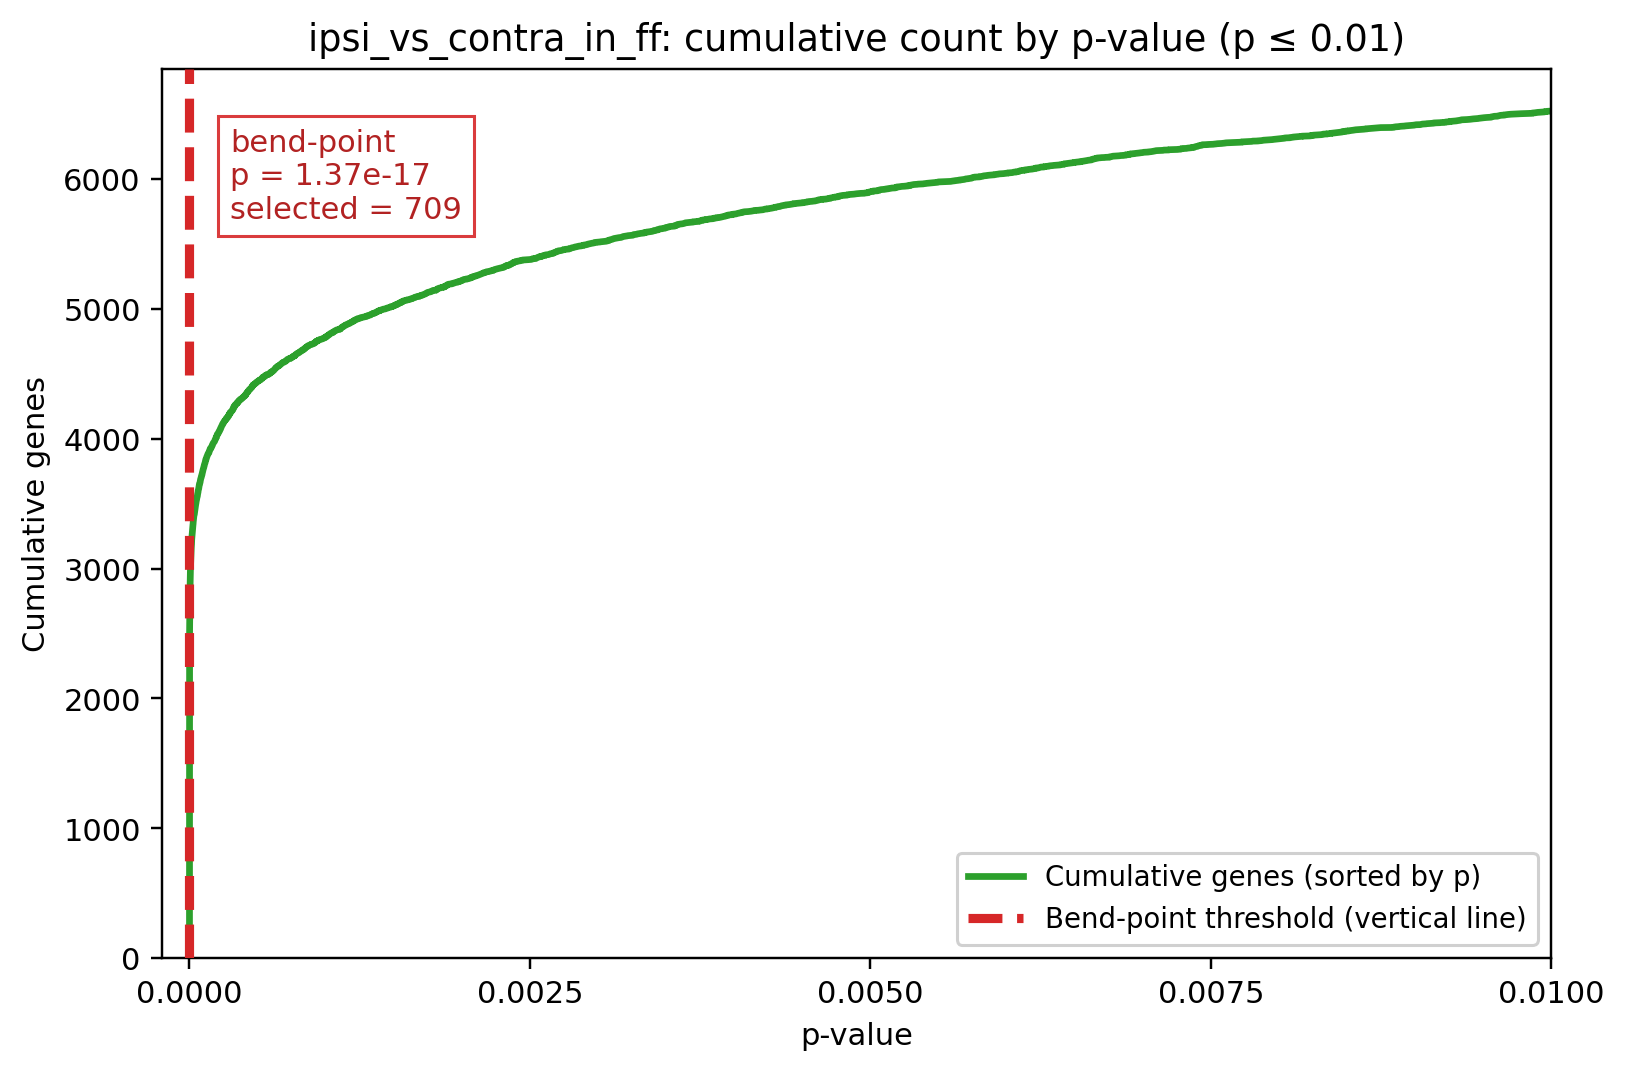
\includegraphics[width=\linewidth,height=0.66\textheight,keepaspectratio]{assets_pca_to_go/ordered_pvalue_cumulative_zoom_p0_0.01.png}

  \column{0.30\textwidth}
  \scriptsize
  \begin{itemize}
    \item Many significant genes $\Rightarrow$ picking a GO input list can feel arbitrary (``top $N$'').
    \item Use an elbow/bend-point cutoff on sorted p-values (where the curve changes slope).
    \item Here: bend-point $p\approx 1.37\times 10^{-17}$ selects $709$ genes (enrichment input).
  \end{itemize}
\end{columns}
\end{frame}

\begin{frame}{Volcano plots: before vs. after selection}
\centering
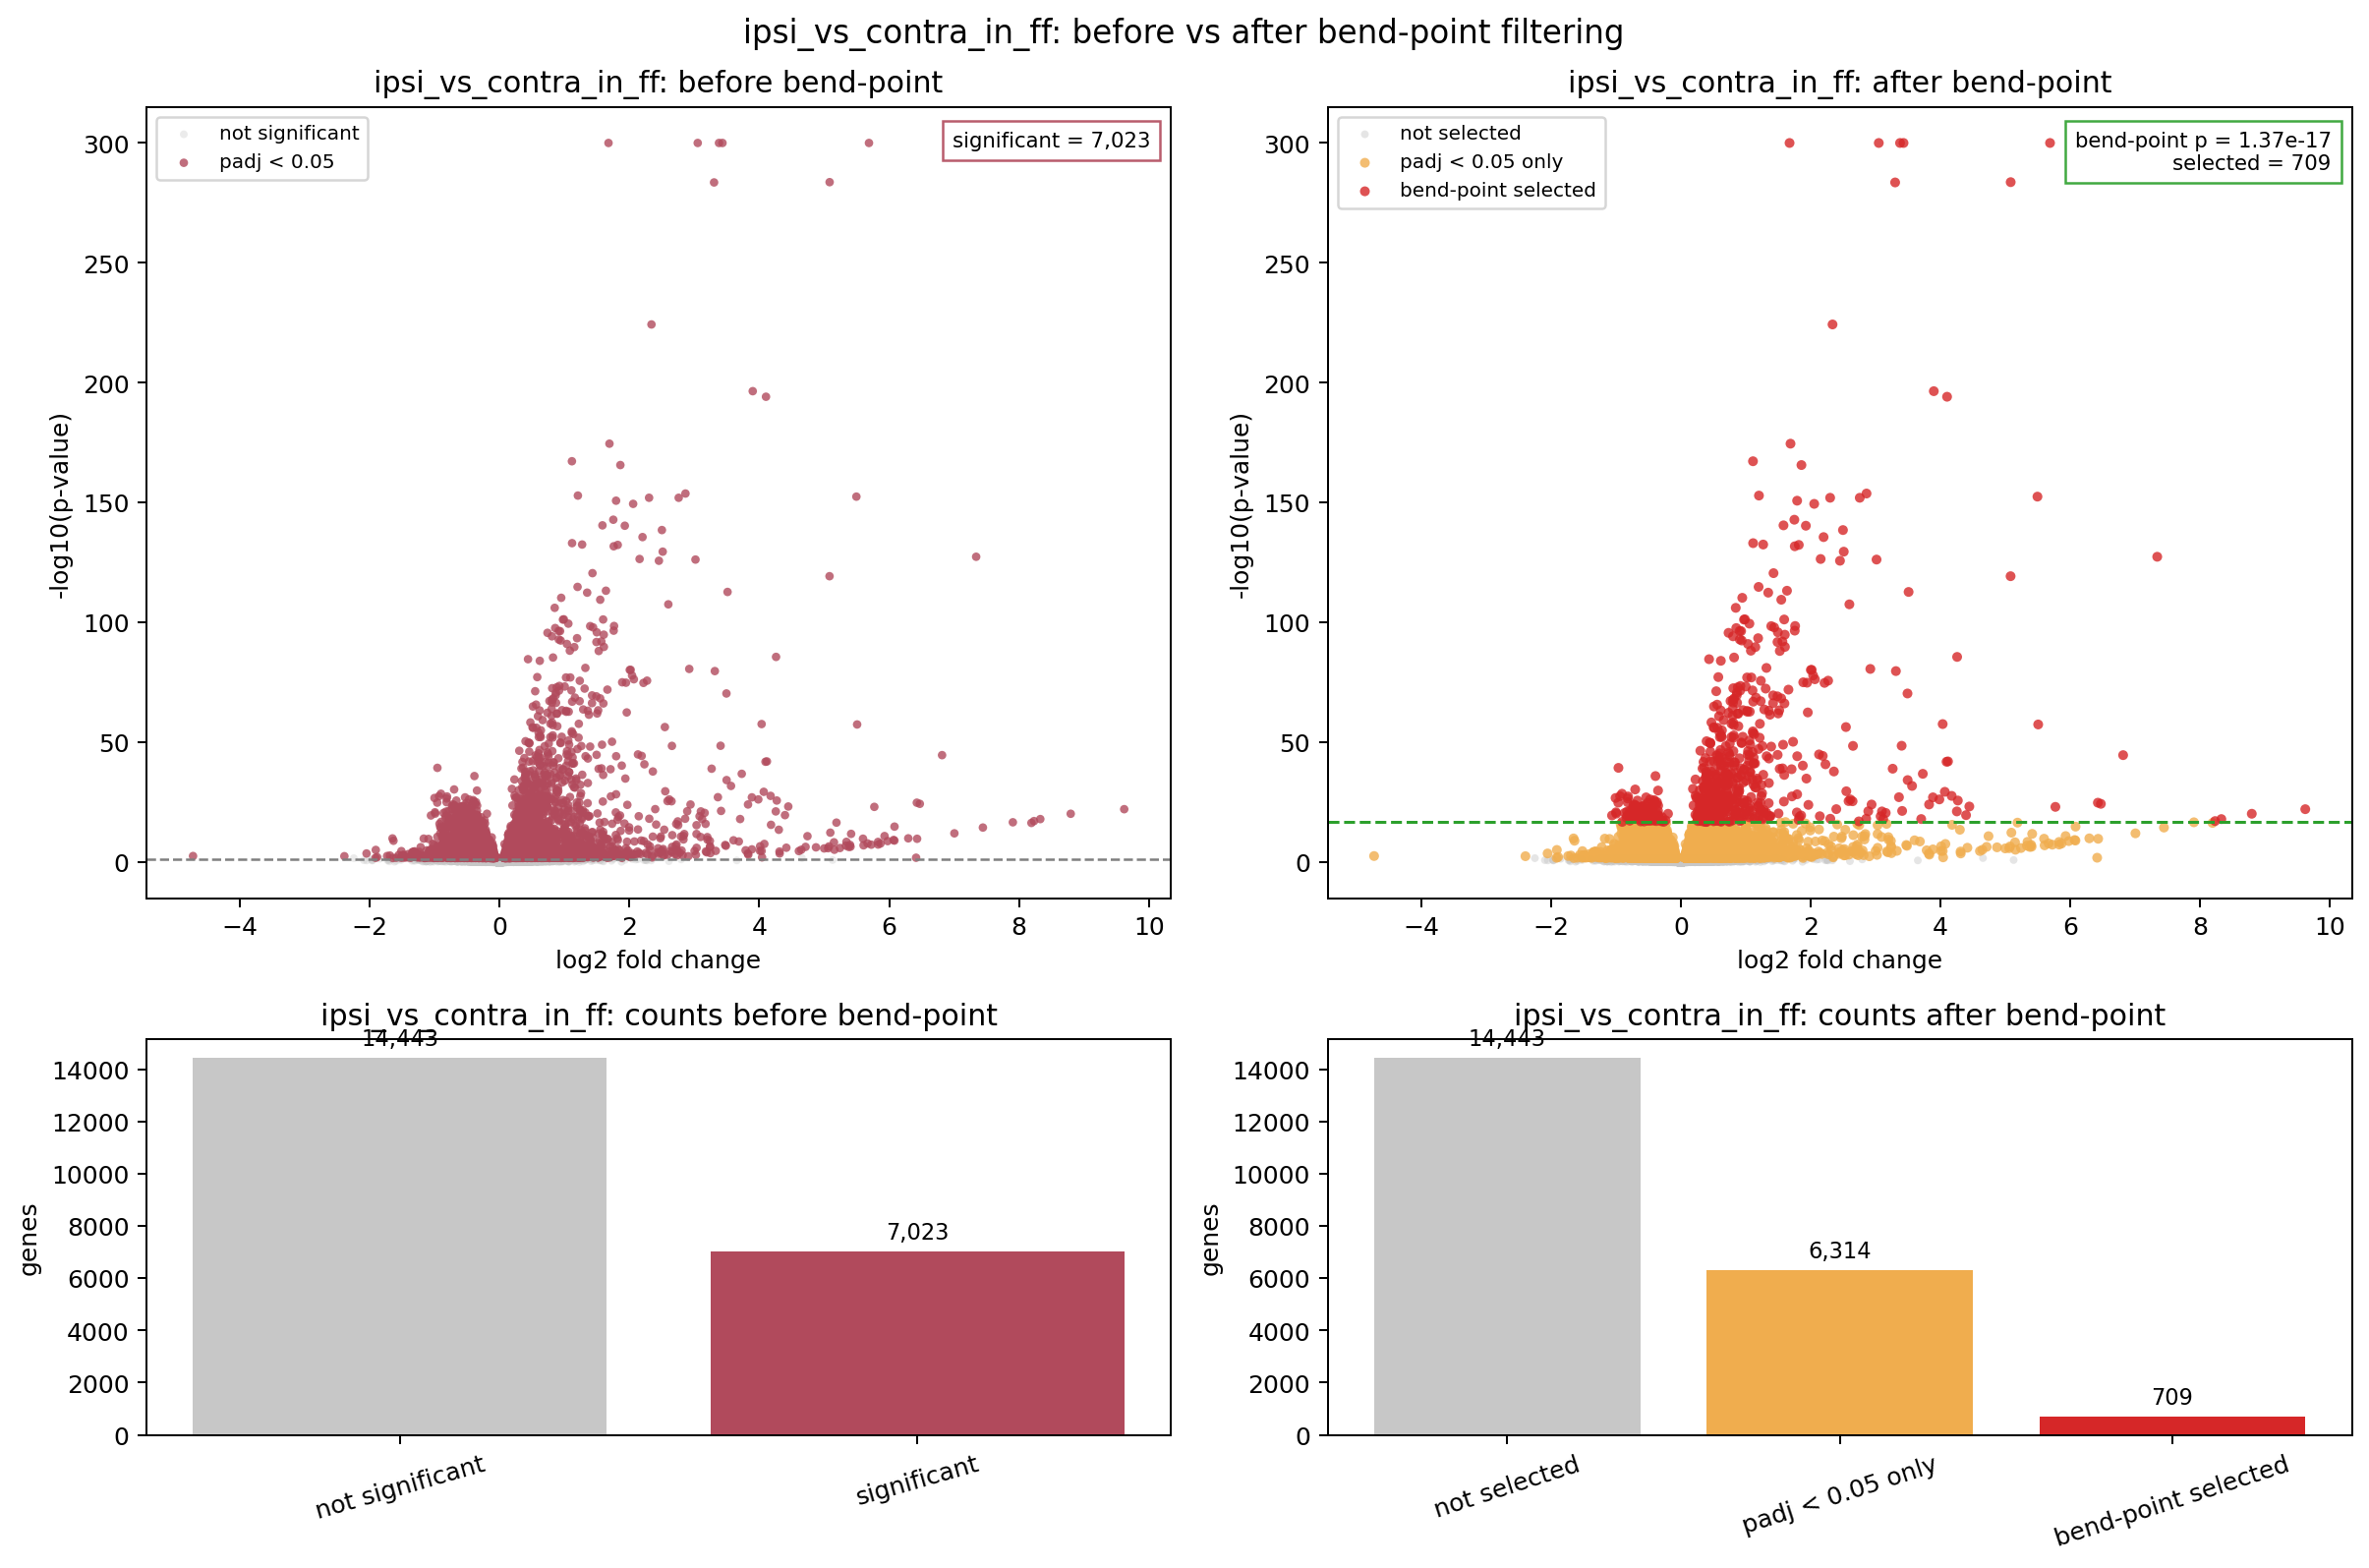
\includegraphics[width=0.95\linewidth,height=0.62\textheight,keepaspectratio]{../data/differential_expression_all20/derived_analysis/ipsi_vs_contra_in_ff/before_after_selection_comparison.png}

\vspace{0pt}
\small
\begin{itemize}
  \item Each point is a gene: $x=\log_2(\text{fold change})$, $y=-\log_{10}(\text{FDR-adjusted }p)$.
  \item Left: all genes; Right: the subset kept after the bend-point cutoff (used as input for enrichment).
  \item Next: run GO/KEGG/Reactome enrichment on this selected gene set to summarize biological themes.
\end{itemize}
\end{frame}

\begin{frame}[fragile]{How we ran it (minimal)}
\scriptsize
\textbf{Input gene list:} \texttt{selected\_genes\_bendpoint.tsv} (\texttt{selected\_by\_bend=True}; $709$ genes; $657$ mapped IDs used by g:Profiler)

\vspace{0.1em}
\textbf{Enrichment call (from \texttt{\detokenize{mouse_new/scripts/derive_de_analysis_all20.py}}):}

\vspace{0.1em}
\begin{lstlisting}[language=Python,basicstyle=\ttfamily\scriptsize]
import requests

def call_gprofiler(gene_ids):
    url = "https://biit.cs.ut.ee/gprofiler/api/gost/profile/"
    payload = {
        "organism": "mmusculus",
        "query": gene_ids,
        "sources": ["GO:BP", "KEGG", "REAC"],
        "user_threshold": 0.05,  # term-level cutoff
    }
    return requests.post(url, json=payload).json()
\end{lstlisting}

\vspace{0.1em}
\textbf{Outputs:} \url{data/differential_expression_all20/derived_analysis/ipsi_vs_contra_in_ff/gprofiler_enrichment.tsv}
\end{frame}

\begin{frame}{GO enrichment: top terms + overlap}
\centering
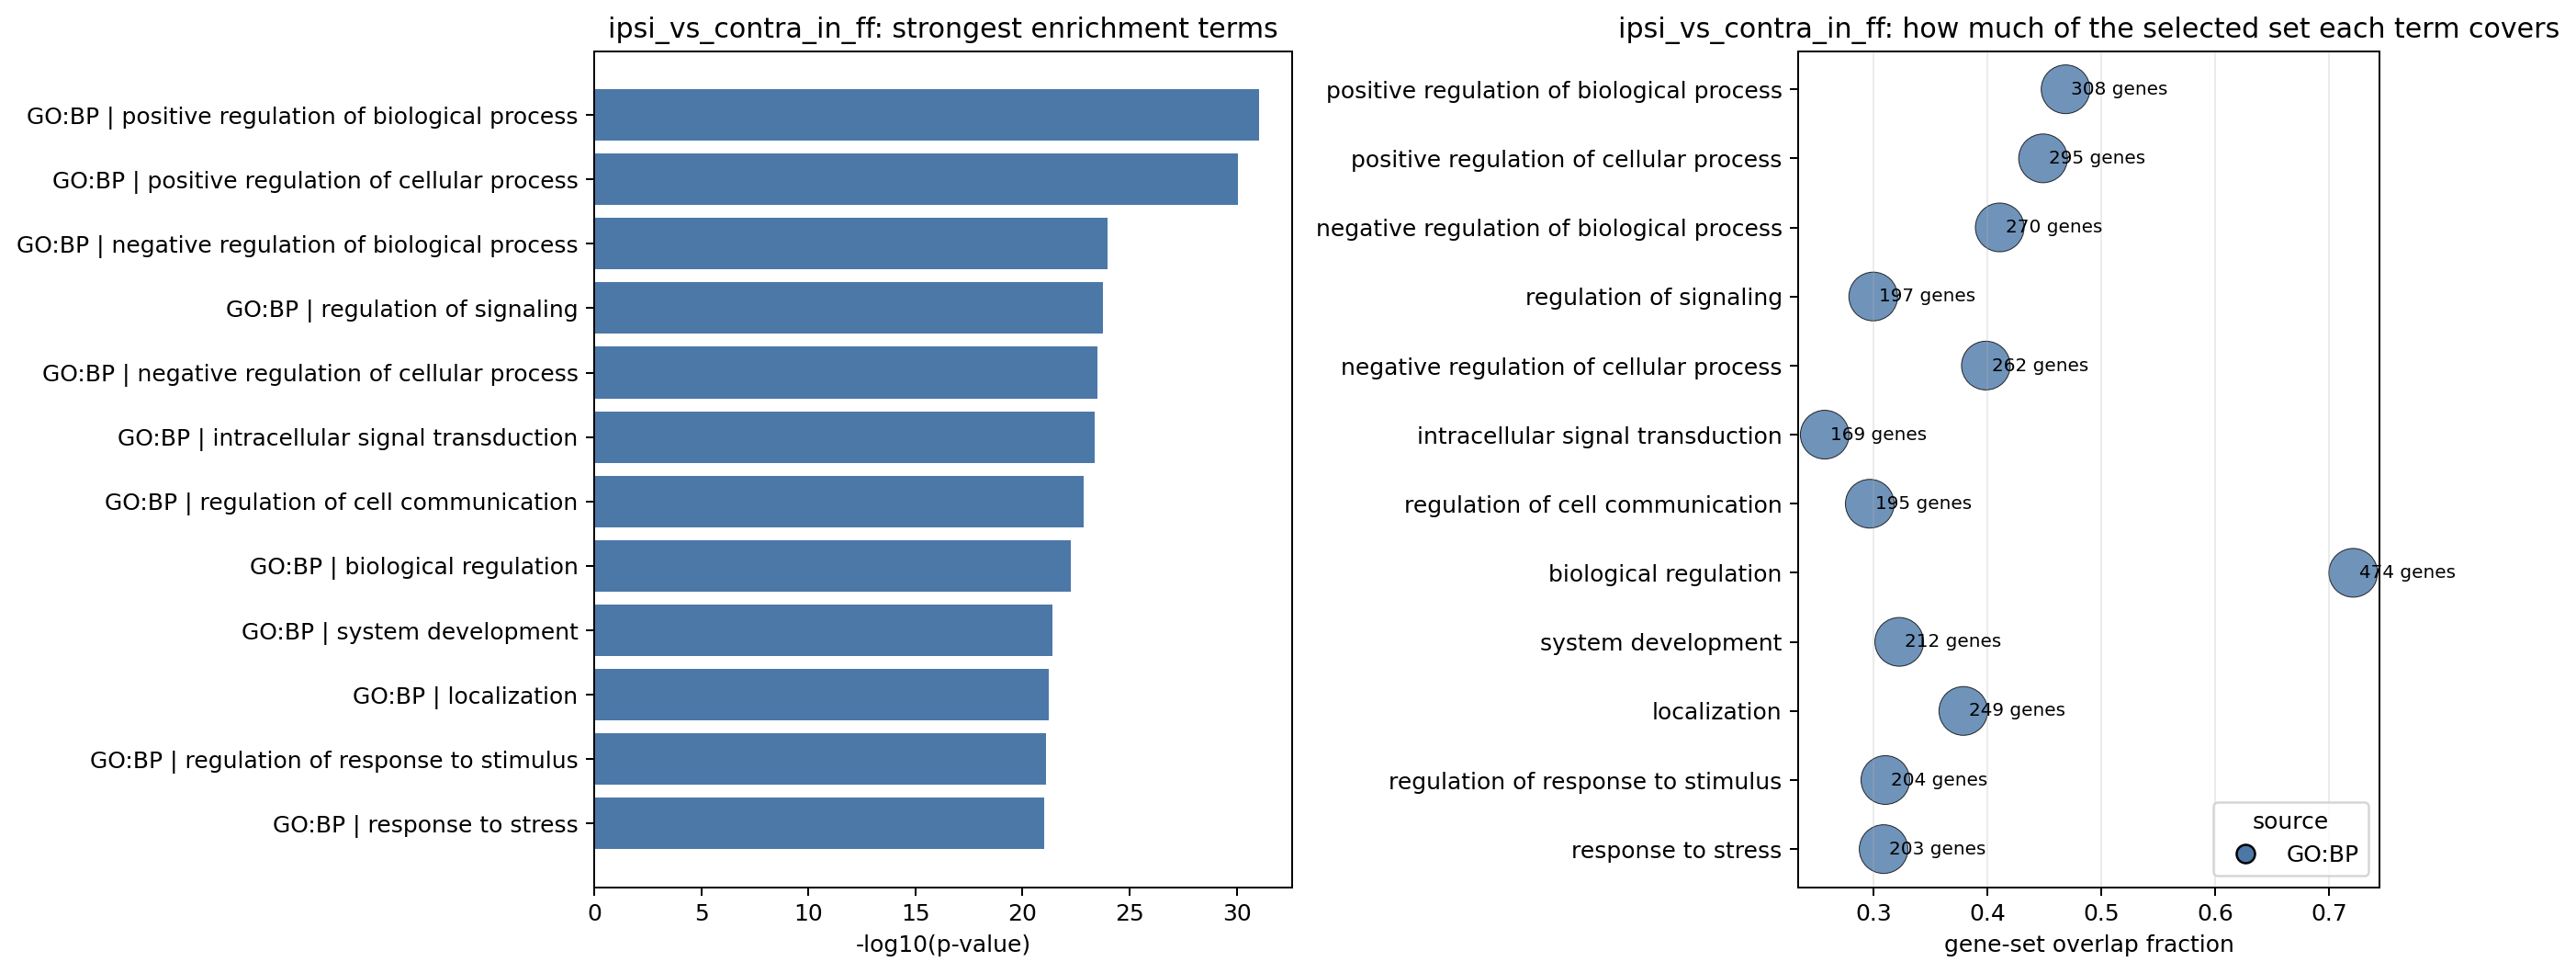
\includegraphics[width=0.98\linewidth,height=0.74\textheight,keepaspectratio]{../data/differential_expression_all20/derived_analysis/ipsi_vs_contra_in_ff/gprofiler_terms_and_overlap.png}

\vspace{0.2em}
\scriptsize
\begin{itemize}
  \item Left: top enriched terms ranked by corrected significance (smaller adjusted $p$ = stronger signal).
  \item Right: term overlap helps distinguish redundant terms vs. distinct functional themes.
\end{itemize}
\end{frame}

\begin{frame}{GO enrichment: sources (GO:BP / KEGG / REAC)}
\centering
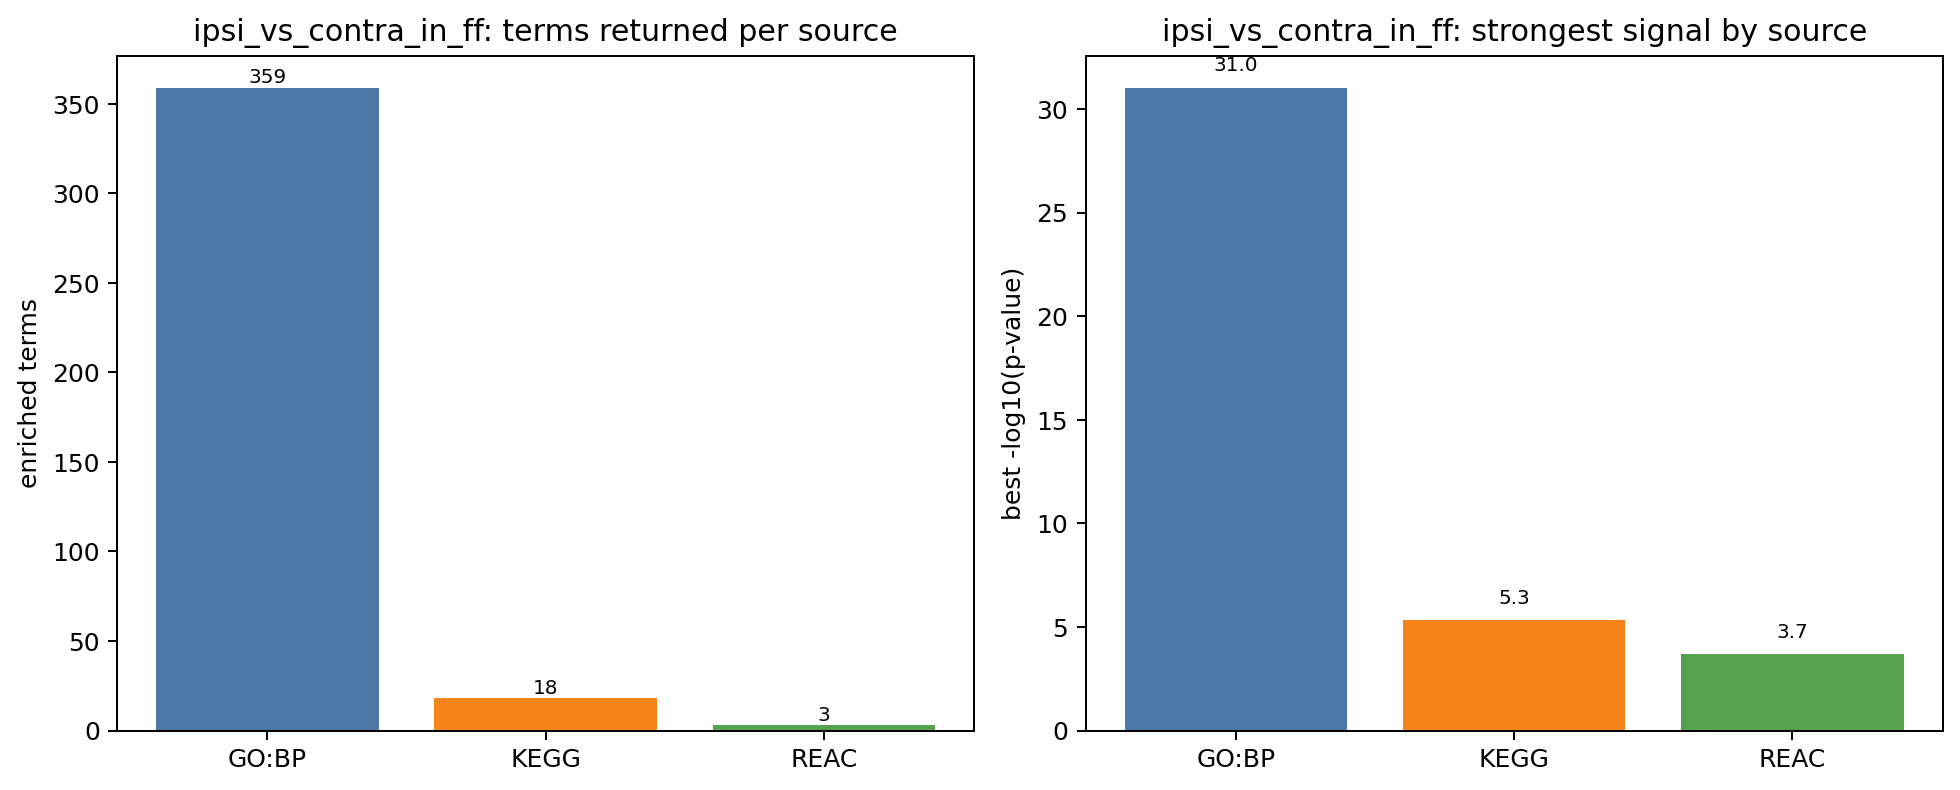
\includegraphics[width=0.98\linewidth,height=0.82\textheight,keepaspectratio]{../data/differential_expression_all20/derived_analysis/ipsi_vs_contra_in_ff/gprofiler_source_summary.png}

\vspace{0.1em}
\footnotesize
\begin{itemize}
  \item Terms are filtered at corrected $p<0.05$ (term-level cutoff), using the bend-point gene set as input.
\end{itemize}
\end{frame}

\begin{frame}{What do GO enrichment p-values mean?}
\small
\begin{itemize}
  \item For each GO term, ask: are term-annotated genes \emph{over-represented} in our query list?
  \item Common model: hypergeometric (Fisher's exact test).
\end{itemize}

\vspace{0.3em}
\small
\begin{align*}
X &\sim \text{Hypergeometric}(N, M, n) \\
\text{p-value} &= P(X \ge k)
\end{align*}

\vspace{-0.2em}
\small
\begin{itemize}
  \item $N$ = background genes with annotations (``effective domain size''), $M$ = term size, $n$ = query size, $k$ = overlap.
  \item Many terms are tested $\Rightarrow$ use multiple-testing correction (FDR / adjusted p-values).
  \item Rule of thumb: testing 1000 terms at $\alpha=0.05$ yields \,$\approx 50$\, false positives by chance.
  \item Enrichment \emph{does not} prove causality; it flags shared functional themes among the genes that changed.
\end{itemize}
\end{frame}

\end{document}
